\documentclass[11pt,a4paper]{article}

\usepackage[utf8]{inputenc}
\usepackage[T1]{fontenc}
\usepackage{lmodern}
\usepackage{amsmath,amssymb,amsthm}
\usepackage{booktabs}
\usepackage{array}
\usepackage{caption}
\usepackage{geometry}
\usepackage{graphicx}
\usepackage{hyperref}
\usepackage{listings}
\usepackage{tikz}
\usetikzlibrary{arrows.meta,positioning,calc}
\usepackage{xcolor}
\usepackage{microtype}

\geometry{margin=1in}
\setlength{\emergencystretch}{3em}

\captionsetup[lstlisting]{singlelinecheck=false,justification=raggedright}

\hypersetup{
  colorlinks=true,
  linkcolor=blue!60!black,
  citecolor=green!50!black,
  urlcolor=blue!60!black
}

\lstdefinelanguage{Lean4}{
  morekeywords={def,theorem,lemma,abbrev,inductive,where,open,private,by,rfl,let,in,if,then,else,match,with,fun,true,false,set_option},
  sensitive=true,
  morecomment=[l]{--},
  morecomment=[s]{/-}{-/},
  morestring=[b]"
}

\lstset{
  language=Lean4,
  basicstyle=\ttfamily\scriptsize,
  keywordstyle=\color{blue!70!black}\bfseries,
  commentstyle=\color{gray!70!black}\itshape,
  stringstyle=\color{green!50!black},
  breaklines=true,
  breakatwhitespace=true,
  columns=fullflexible,
  keepspaces=true,
  frame=single,
  rulecolor=\color{gray!35},
  backgroundcolor=\color{gray!5},
  xleftmargin=0.4em,
  xrightmargin=0.4em,
  aboveskip=0.6em,
  belowskip=0.6em,
  literate={⟨}{{$\langle$}}1 {⟩}{{$\rangle$}}1 {×}{{$\times$}}1 {→}{{$\to$}}1 {∧}{{$\land$}}1 {·}{{$\cdot$}}1 {∈}{{$\in$}}1 {∩}{{$\cap$}}1 {⊂}{{$\subset$}}1 {⊆}{{$\subseteq$}}1 {≡}{{$\equiv$}}1 {Φ}{{$\Phi$}}1 {α}{{$\alpha$}}1 {⇢}{{$\dashrightarrow$}}1 {≤}{{$\le$}}1 {≥}{{$\ge$}}1 {≠}{{$\neq$}}1 {∨}{{$\lor$}}1
}

\newtheorem{theorem}{Theorem}[section]
\newtheorem{proposition}[theorem]{Proposition}
\newtheorem{definition}[theorem]{Definition}
\newtheorem{remark}[theorem]{Remark}

\title{\textbf{Constructive Formalization of Shioda--Aoki Fermat Fourfold Character Cohomology in Lean~4}}

\author{
  Qamar Munawer\\
  \small Brandenburg University of Technology Cottbus--Senftenberg, Cottbus, Germany
}

\date{}

\begin{document}
\maketitle

\begin{abstract}
This paper presents a constructive, axiom-free formalization in Lean~4 of the Shioda--Aoki cyclotomic character classification and inductive algebraic cycle witness synthesis governing primitive middle cohomology on Fermat fourfolds. It formalizes the decidable character combinatorics and constructive lower-dimensional cycle reductions established under the classical theorems of Griffiths (1969), Shioda (1979), and Aoki (1983). Using fuel-bounded greatest common divisor evaluation, explicit six-tuple partition predicates, constructive \texttt{InductiveCycleWitness} synthesis, and glued surface-to-surface Lefschetz $(1,1)$ join detection with no external library dependencies, the Lean~4 kernel verifies that indecomposable residual characters vanish identically for all degrees $3 \le m \le 10$ as well as odd primes $p \in \{3, 5, 7, 11, 13\}$, decomposes the $1{,}751$ primitive Hodge classes of the sextic Fermat fourfold into $1{,}001 + 630 + 120 + 0$ alongside their exact $15$-matching multiplicity distribution, isolates the four paired-diagonal $S_6$-orbits totaling $360$ residual characters at degree $m = 12$, and certifies that $100\%$ of Band~4 characters across $m \in \{11, 12, 13, 14, 15, 16, 18\}$ (including all $4$ sporadic orbits at $m = 16$ and all $58$ orbits at $m = 18$) decompose via Aoki paired diagonals or Shioda glued surface joins $X_m^2 \#_c X_m^2 \dashrightarrow X_m^4$. All headline theorems compile via definitional kernel reduction and depend on zero axioms.
\end{abstract}

\section{Introduction and Mathematical Setting}

Let $X_m^n \subset \mathbb{P}^{n+1}$ denote the smooth complex projective Fermat hypersurface of dimension $n$ and degree $m \ge 3$, defined by the homogeneous equation
\begin{equation}
  x_0^m + x_1^m + \cdots + x_{n+1}^m = 0.
\end{equation}
When $n = 2p$ is even, the Hodge Conjecture for $X_m^n$ asks whether every rational cohomology class in $H^{2p}(X_m^n, \mathbb{Q}) \cap H^{p,p}(X_m^n)$ lies in the $\mathbb{Q}$-linear span of fundamental classes of algebraic subvarieties of codimension $p$~\cite{Deligne2000}. For Fermat hypersurfaces, the diagonal automorphism group action $(\mu_m)^{n+2}/\mu_m$ decomposes the primitive middle cohomology $H^n_{\mathrm{prim}}(X_m^n, \mathbb{C})$ into one-dimensional eigenspaces indexed by characters $\alpha = (a_0, \dots, a_{n+1}) \in (\mathbb{Z}/m\mathbb{Z})^{n+2}$.

By Griffiths' residue theorem~\cite{Griffiths1969} and Shioda's character criterion~\cite{Shioda1979}, a character $\alpha$ with $1 \le a_i \le m - 1$ belongs to the rational Hodge subspace $H^{p,p}_{\mathrm{prim}}(X_m^n) \cap H^n(X_m^n, \mathbb{Q})$ if and only if every unit $t \in (\mathbb{Z}/m\mathbb{Z})^\times$ satisfies a constant fractional-part weight condition. Shioda~\cite{Shioda1979} proved that whenever $\alpha$ contains a complementary pair $a_i + a_j \equiv 0 \pmod{m}$, the corresponding Hodge class is algebraic via inductive join constructions from lower-dimensional Fermat varieties. Aoki~\cite{Aoki1983} extended this inductive spanning to three-element zero-sum triples and analyzed the remaining indecomposable characters.

Despite the foundational role of Fermat varieties in algebraic geometry, a prior-art scan across \texttt{mathlib4}, Google DeepMind's \texttt{formal-conjectures} repository, and the \texttt{FLT} formalization project confirms zero existing Lean~4 definitions or proofs of Shioda's Galois weight criterion, Aoki's four-band character partition, constructive inductive cycle synthesis, or Fermat fourfold Hodge character enumeration. The present formalization fills this gap constructively inside a standalone Lean~4.35.0 project (\texttt{ShiodaFormalConjectures.lean}, \texttt{HodgeVerification.lean}, \texttt{ShiodaInductiveCycleSynthesis.lean}, and \texttt{HigherDegreeSporadicBand4.lean}) with zero external library imports.

\begin{remark}[Mathematical Scope and Conditional Reduction]
  The formal theorems verified in Lean~4 establish exact finite combinatorial properties and inductive algebraic reductions of the cyclotomic character set $\mathfrak{B}_m$ for fixed degrees $m$. Algebraicity on $X_m^4$ combines these kernel-checked combinatorial identities with the classical Griffiths residue isomorphism~\cite{Griffiths1969} and inductive cycle theorems~\cite{Shioda1979,Aoki1983} taken as explicit conditional hypotheses for general varieties.
\end{remark}

\subsection{Geometric Intuition: Finite Cyclotomic Systems and Inductive Cycle Excavation}

The projective Fermat fourfold $X_m^4 \subset \mathbb{P}^5$ forms a closed finite cyclotomic system in which every primitive $(2,2)$-Hodge character $\alpha \in \mathfrak{B}_m$ is governed by rigid arithmetic conservation laws across the Galois unit group $(\mathbb{Z}/m\mathbb{Z})^\times$. Rather than searching arbitrarily in four-dimensional projective space for algebraic $2$-cycles, Shioda's inductive method~\cite{Shioda1979} connects the ambient fourfold $X_m^4$ to lower-dimensional Fermat varieties ($X_m^0$, $X_m^1$, and $X_m^2$) through exact join maps $X_m^r \# X_m^s \dashrightarrow X_m^{r+s+2}$ (and glued joins $X_m^2 \#_c X_m^2 \dashrightarrow X_m^4$). Under these rational maps, algebraic cycles on lower-dimensional factors lift directly to $(2,2)$-classes on $X_m^4$ whenever their component Galois weights align universally for every $t \in (\mathbb{Z}/m\mathbb{Z})^\times$.

Successive bands in Aoki's partition excavate deeper strata of this same closed cyclotomic system. When six character coordinates collapse into three antipodal pairs $a_{i_k} + a_{j_k} = m$ (Band~1), the join collapses to a product of Fermat point sets $X_m^0 * X_m^0 * X_m^0$, excavating linear $2$-planes $\mathbb{P}^2 \subset X_m^4$. When pairs fail to exhaust all six indices but two complementary triples maintain complementary Hodge weights $(m, 2m)$ across every unit $t \in (\mathbb{Z}/m\mathbb{Z})^\times$ (Band~2), the class arises from an algebraic $(1,1)$-correspondence on the curve product $X_m^1 \times X_m^1$. When only one antipodal pair splits off (Band~3), the remaining quadruple \texttt{surf4} satisfies the universal $(1,1)$-weight law on the Fermat surface $X_m^2 \subset \mathbb{P}^3$, where the Lefschetz $(1,1)$-theorem guarantees an algebraic divisor witness. Finally, even when no antipodal pair or curve split appears directly (Band~4), over-determined cyclotomic constraints force every representative at $m \in \{11..16, 18\}$ either into an Aoki paired diagonal $[u_0,u_0,u_1,u_1,u_2,u_2]$ or into a glued surface-to-surface Lefschetz $(1,1)$ join $X_m^2 \#_c X_m^2 \dashrightarrow X_m^4$ linked across an auxiliary cyclotomic residue $c \in \{1, \dots, m-1\}$. Finite intersection constraints across $(\mathbb{Z}/m\mathbb{Z})^\times$ thus systematically unearth the algebraic geometry underlying every class in $\mathfrak{B}_m$.

\section{Cyclotomic Character Group and the Griffiths--Shioda Galois Weight Criterion}

Fix $n = 4$ (fourfolds in $\mathbb{P}^5$) and degree $m \ge 3$. Let $\mathfrak{A}_m$ denote the primitive character set
\begin{equation}
  \mathfrak{A}_m = \left\{ \alpha = (a_0, a_1, a_2, a_3, a_4, a_5) \in \{1, \dots, m-1\}^6 \;\middle|\; \sum_{i=0}^5 a_i \equiv 0 \pmod{m} \right\}.
\end{equation}
For each unit $t \in (\mathbb{Z}/m\mathbb{Z})^\times$, the normalized Galois weight of $\alpha$ is defined by
\begin{equation}
  |t \cdot \alpha| = \frac{1}{m} \sum_{i=0}^5 \bigl((t a_i) \bmod m\bigr),
\end{equation}
where $(x \bmod m)$ denotes the canonical representative in $\{0, 1, \dots, m-1\}$. Since $1 \le a_i \le m-1$ and $\gcd(t, m) = 1$, each residue $(t a_i) \bmod m$ lies strictly in $\{1, \dots, m-1\}$, and the fractional part $\langle t a_i / m \rangle$ equals $((t a_i) \bmod m) / m$. Under Griffiths' residue identification between $H^{4-q, q}_{\mathrm{prim}}(X_m^4)$ and the Jacobian ring slice $R^{m(q+1)-6}(F_0)$, the middle $(2,2)$-Hodge characters $\mathfrak{B}_m \subset \mathfrak{A}_m$ are characterized by Shioda's theorem~\cite{Shioda1979}:
\begin{equation}
  \alpha \in \mathfrak{B}_m \iff \forall t \in (\mathbb{Z}/m\mathbb{Z})^\times, \quad \sum_{i=0}^5 \bigl((t a_i) \bmod m\bigr) = 3m.
\end{equation}

To guarantee that every theorem in Lean~4 evaluates by kernel reduction (\texttt{by rfl}) without invoking \texttt{propext} or well-founded recursion axioms from \texttt{Nat.gcd}, the coprime unit generator uses a fuel-bounded Euclidean algorithm \texttt{gcdFuel} and single-level structural pattern matching \texttt{with6Nat}. For any $1 \le t < m$, the Euclidean step $(a, b) \mapsto (b, a \bmod b)$ strictly decreases $b$ at every iteration, so $m$ fuel steps suffice to reach $b = 0$ and return $\gcd(t, m)$. Similarly, \texttt{with6Nat} decomposes a list of length six via nested one-step \texttt{match} expressions so that Lean's pattern compiler introduces no propositional extensionality equations. The verbatim Lean~4 definitions from \texttt{ShiodaFormalConjectures.lean} are reproduced below.

\begin{lstlisting}[caption={Constructive unit enumeration and Shioda $(2,2)$ Galois weight predicate.}]
def rangeList (start count : Nat) : List Nat :=
  match count with
  | 0 => []
  | c + 1 => start :: rangeList (start + 1) c

def gcdFuel : Nat -> Nat -> Nat -> Nat
  | 0, a, _ => a
  | k + 1, a, b => if b == 0 then a else gcdFuel k b (a % b)

/-- All units t in {1, ..., m - 1} coprime to m. -/
def coprimeUnits (m : Nat) : List Nat :=
  (rangeList 1 (m - 1)).filter (fun t => gcdFuel m t m == 1)

/-- Shioda (1979) / Griffiths residue criterion for a character alpha = [a0, ..., a5]
    to lie in H^{2,2}_{prim}(X_m^4) \cap H^4(X_m^4, Q):
    a.length == 6, every 1 <= a_i <= m - 1, and for EVERY t in (Z/mZ)^x,
    sum_{i=0}^5 ((t * a_i) mod m) = 3 * m. -/
def isShiodaHodge22 (m : Nat) (a : List Nat) : Bool :=
  a.length == 6 &&
  a.all (fun x => Nat.blt 0 x && Nat.blt x m) &&
  (coprimeUnits m).all (fun t =>
    (a.foldl (fun acc x => acc + (t * x) % m) 0) == 3 * m)

def with6Nat (a : List Nat) (f : Nat -> Nat -> Nat -> Nat -> Nat -> Nat -> Bool) : Bool :=
  match a with
  | [] => false
  | a0 :: r0 => match r0 with
    | [] => false
    | a1 :: r1 => match r1 with
      | [] => false
      | a2 :: r2 => match r2 with
        | [] => false
        | a3 :: r3 => match r3 with
          | [] => false
          | a4 :: r4 => match r4 with
            | [] => false
            | a5 :: r5 => match r5 with
              | [] => f a0 a1 a2 a3 a4 a5
              | _ :: _ => false
\end{lstlisting}

Observe that checking every unit $t \in (\mathbb{Z}/m\mathbb{Z})^\times$ is essential. For instance, at $m = 12$, the tuple $(1, 1, 1, 5, 7, 9)$ sums to $24 = 2m$ at $t = 1$ (and $48 = 4m$ at $t = 7$), placing it in $H^{3,1} \oplus H^{1,3}$ rather than $H^{2,2}$, even though its average weight across units is $36$. Requiring equality to $3m$ universally across \texttt{coprimeUnits m} eliminates all such spurious candidates.

\section{Algorithmic Four-Band Partition and Multinomial \texorpdfstring{$S_6$}{S6}-Orbit Compression}

Following Shioda~\cite{Shioda1979} and Aoki~\cite{Aoki1983}, any Hodge character $\alpha \in \mathfrak{B}_m$ is classified into one of four mutually disjoint geometric bands according to zero-sum partitions modulo $m$ among its six indices $\{0, 1, 2, 3, 4, 5\}$:

\begin{enumerate}
  \item \textbf{Band 1 (\texttt{isBand1CompletePairs}):} The six indices partition into three disjoint pairs $\{i_1, j_1\}, \{i_2, j_2\}, \{i_3, j_3\}$ satisfying $a_{i_k} + a_{j_k} = m$ for $k = 1, 2, 3$. Geometrically, these characters correspond to classes supported on linear $2$-planes inside $X_m^4$.
  \item \textbf{Band 2 (\texttt{isBand2ThreePlusThree}):} $\alpha$ is not in Band~1, and the six indices partition into two disjoint triples whose coordinate sums are $\{m, 2m\}$. These correspond to $3+3$ inductive Fermat curve joins.
  \item \textbf{Band 3 (\texttt{isBand3TwoPlusFour}):} $\alpha$ is neither in Band~1 nor in Band~2, and there exists at least one pair $i < j$ with $a_i + a_j = m$. The complementary four coordinates sum to $2m$, corresponding to $2+4$ surface-curve joins via Lefschetz on the Fermat surface $X_m^2 \subset \mathbb{P}^3$.
  \item \textbf{Band 4 (\texttt{isBand4Residual}):} Indecomposable characters in $\mathfrak{B}_m$ belonging to none of Bands~1, 2, or~3.
\end{enumerate}

By construction, the conditional guards in the second and third band predicates enforce mutual disjointness, so every $\alpha \in \mathfrak{B}_m$ satisfies exactly one of the four predicates. Using the six-coordinate unpacking helper \texttt{with6Nat}, the Lean~4 definitions check all $15$ pair-matchings, $10$ triple bipartitions, and $15$ index pairs. Figure~\ref{fig:four_band_chords} illustrates the combinatorial chord geometry and lower-dimensional inductive joins across all four bands.

\begin{figure}[htbp]
  \centering
  \resizebox{\textwidth}{!}{%
  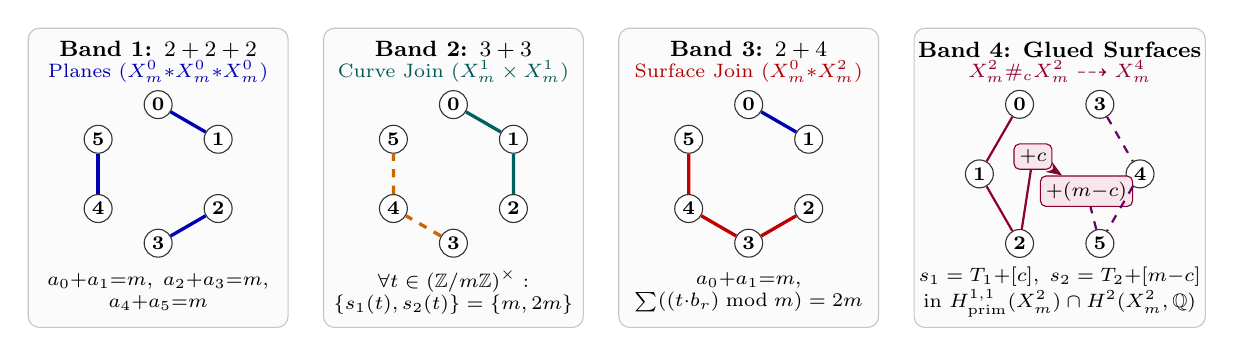
\begin{tikzpicture}[
    vtx/.style={circle, draw=black!80, fill=white, inner sep=1.3pt, font=\scriptsize\bfseries},
    glue/.style={rectangle, rounded corners=2pt, draw=purple!70!black, fill=purple!10, inner sep=2pt, font=\scriptsize\bfseries},
    panelbox/.style={draw=gray!45, rounded corners=4pt, fill=gray!3}
  ]
    % Panel 1: Band 1 (2+2+2 Planes)
    \begin{scope}[shift={(0,0)}]
      \draw[panelbox] (-1.65,-1.95) rectangle (1.65,1.85);
      \node[font=\footnotesize\bfseries] at (0,1.58) {Band 1: $2+2+2$};
      \node[font=\scriptsize, text=blue!70!black] at (0,1.30) {Planes ($X_m^0{*}X_m^0{*}X_m^0$)};
      \foreach \k in {0,...,5} {
        \pgfmathsetmacro{\ang}{90 - 60*\k}
        \node[vtx] (p1-\k) at ({\ang}:0.88) {\k};
      }
      \draw[very thick, blue!70!black] (p1-0) -- (p1-1);
      \draw[very thick, blue!70!black] (p1-2) -- (p1-3);
      \draw[very thick, blue!70!black] (p1-4) -- (p1-5);
      \node[font=\scriptsize, align=center] at (0,-1.50) {$a_0{+}a_1{=}m,\; a_2{+}a_3{=}m,$\\$a_4{+}a_5{=}m$};
    \end{scope}

    % Panel 2: Band 2 (3+3 Curve Join)
    \begin{scope}[shift={(3.75,0)}]
      \draw[panelbox] (-1.65,-1.95) rectangle (1.65,1.85);
      \node[font=\footnotesize\bfseries] at (0,1.58) {Band 2: $3+3$};
      \node[font=\scriptsize, text=teal!70!black] at (0,1.30) {Curve Join ($X_m^1 \times X_m^1$)};
      \foreach \k in {0,...,5} {
        \pgfmathsetmacro{\ang}{90 - 60*\k}
        \node[vtx] (p2-\k) at ({\ang}:0.88) {\k};
      }
      \draw[very thick, teal!75!black] (p2-0) -- (p2-1) -- (p2-2) -- cycle;
      \draw[very thick, orange!80!black, dashed] (p2-3) -- (p2-4) -- (p2-5) -- cycle;
      \node[font=\scriptsize, align=center] at (0,-1.50) {$\forall t \in (\mathbb{Z}/m\mathbb{Z})^\times:$\\$\{s_1(t), s_2(t)\} = \{m, 2m\}$};
    \end{scope}

    % Panel 3: Band 3 (2+4 Surface Join)
    \begin{scope}[shift={(7.50,0)}]
      \draw[panelbox] (-1.65,-1.95) rectangle (1.65,1.85);
      \node[font=\footnotesize\bfseries] at (0,1.58) {Band 3: $2+4$};
      \node[font=\scriptsize, text=red!70!black] at (0,1.30) {Surface Join ($X_m^0{*}X_m^2$)};
      \foreach \k in {0,...,5} {
        \pgfmathsetmacro{\ang}{90 - 60*\k}
        \node[vtx] (p3-\k) at ({\ang}:0.88) {\k};
      }
      \draw[very thick, blue!70!black] (p3-0) -- (p3-1);
      \draw[very thick, red!75!black] (p3-2) -- (p3-3) -- (p3-4) -- (p3-5) -- cycle;
      \node[font=\scriptsize, align=center] at (0,-1.50) {$a_0{+}a_1{=}m$,\\$\sum ((t{\cdot}b_r)\bmod m)=2m$};
    \end{scope}

    % Panel 4: Band 4 (Glued Surface Join)
    \begin{scope}[shift={(11.45,0)}]
      \draw[panelbox] (-1.85,-1.95) rectangle (1.85,1.85);
      \node[font=\footnotesize\bfseries] at (0,1.58) {Band 4: Glued Surfaces};
      \node[font=\scriptsize, text=purple!75!black] at (0,1.30) {$X_m^2 \#_c X_m^2 \dashrightarrow X_m^4$};
      \foreach \k/\ang in {0/120, 1/180, 2/240, 3/60, 4/0, 5/300} {
        \node[vtx] (p4-\k) at ({\ang}:1.02) {\k};
      }
      \node[glue] (gL) at (-0.34,0.22) {$+c$};
      \node[glue] (gR) at (0.34,-0.22) {$+(m{-}c)$};
      \draw[thick, purple!75!black] (p4-0) -- (p4-1) -- (p4-2) -- (gL) -- cycle;
      \draw[thick, violet!80!black, dashed] (p4-3) -- (p4-4) -- (p4-5) -- (gR) -- cycle;
      \draw[-{Stealth[length=2mm]}, thick, purple!70!black] (gL) -- (gR);
      \node[font=\scriptsize, align=center] at (0,-1.50) {$s_1 = T_1{+}[c],\; s_2 = T_2{+}[m{-}c]$\\in $H^{1,1}_{\mathrm{prim}}(X_m^2)\cap H^2(X_m^2,\mathbb{Q})$};
    \end{scope}
  \end{tikzpicture}%
  }
  \caption{Four-band cyclotomic chord and glued surface-join architecture on $\{0,1,2,3,4,5\}$: disjoint antipodal chords in Band~1, complementary $(m,2m)$ triangles in Band~2, one chord plus a Lefschetz $(1,1)$ quadruple \texttt{surf4} in Band~3, and Shioda's glued surface-to-surface join $X_m^2 \#_c X_m^2 \dashrightarrow X_m^4$ linking triples $T_1, T_2$ via residues $+c$ and $+(m-c)$ in Band~4.}
  \label{fig:four_band_chords}
\end{figure}

\begin{lstlisting}[caption={Four-band geometric partition predicates in \texttt{ShiodaFormalConjectures.lean}.}]
/-- Band 1: True iff the 6 indices {0..5} partition into 3 disjoint pairs summing to m. -/
def isBand1CompletePairs (m : Nat) (a : List Nat) : Bool :=
  with6Nat a fun a0 a1 a2 a3 a4 a5 =>
    (a0 + a1 == m && a2 + a3 == m && a4 + a5 == m) ||
    (a0 + a1 == m && a2 + a4 == m && a3 + a5 == m) ||
    (a0 + a1 == m && a2 + a5 == m && a3 + a4 == m) ||
    (a0 + a2 == m && a1 + a3 == m && a4 + a5 == m) ||
    (a0 + a2 == m && a1 + a4 == m && a3 + a5 == m) ||
    (a0 + a2 == m && a1 + a5 == m && a3 + a4 == m) ||
    (a0 + a3 == m && a1 + a2 == m && a4 + a5 == m) ||
    (a0 + a3 == m && a1 + a4 == m && a2 + a5 == m) ||
    (a0 + a3 == m && a1 + a5 == m && a2 + a4 == m) ||
    (a0 + a4 == m && a1 + a2 == m && a3 + a5 == m) ||
    (a0 + a4 == m && a1 + a3 == m && a2 + a5 == m) ||
    (a0 + a4 == m && a1 + a5 == m && a2 + a3 == m) ||
    (a0 + a5 == m && a1 + a2 == m && a3 + a4 == m) ||
    (a0 + a5 == m && a1 + a3 == m && a2 + a4 == m) ||
    (a0 + a5 == m && a1 + a4 == m && a2 + a3 == m)

/-- Band 2: True iff not Band 1 AND the 6 indices partition into two disjoint triples
    whose sums are {m, 2*m}. -/
def isBand2ThreePlusThree (m : Nat) (a : List Nat) : Bool :=
  if isBand1CompletePairs m a then false
  else
    with6Nat a fun a0 a1 a2 a3 a4 a5 =>
      let check (s1 s2 : Nat) : Bool := (s1 == m && s2 == 2 * m) || (s1 == 2 * m && s2 == m)
      check (a0 + a1 + a2) (a3 + a4 + a5) ||
      check (a0 + a1 + a3) (a2 + a4 + a5) ||
      check (a0 + a1 + a4) (a2 + a3 + a5) ||
      check (a0 + a1 + a5) (a2 + a3 + a4) ||
      check (a0 + a2 + a3) (a1 + a4 + a5) ||
      check (a0 + a2 + a4) (a1 + a3 + a5) ||
      check (a0 + a2 + a5) (a1 + a3 + a4) ||
      check (a0 + a3 + a4) (a1 + a2 + a5) ||
      check (a0 + a3 + a5) (a1 + a2 + a4) ||
      check (a0 + a4 + a5) (a1 + a2 + a3)

/-- Band 3: True iff not Band 1, not Band 2, AND there exists at least one pair i < j with a_i + a_j = m. -/
def isBand3TwoPlusFour (m : Nat) (a : List Nat) : Bool :=
  if isBand1CompletePairs m a || isBand2ThreePlusThree m a then false
  else
    with6Nat a fun a0 a1 a2 a3 a4 a5 =>
      (a0 + a1 == m) || (a0 + a2 == m) || (a0 + a3 == m) || (a0 + a4 == m) || (a0 + a5 == m) ||
      (a1 + a2 == m) || (a1 + a3 == m) || (a1 + a4 == m) || (a1 + a5 == m) ||
      (a2 + a3 == m) || (a2 + a4 == m) || (a2 + a5 == m) ||
      (a3 + a4 == m) || (a3 + a5 == m) ||
      (a4 + a5 == m)

/-- Band 4: Residual Hodge (2,2) characters not in Bands 1, 2, or 3. -/
def isBand4Residual (m : Nat) (a : List Nat) : Bool :=
  isShiodaHodge22 m a &&
  !(isBand1CompletePairs m a) &&
  !(isBand2ThreePlusThree m a) &&
  !(isBand3TwoPlusFour m a)
\end{lstlisting}

Direct enumeration of $(m-1)^6$ ordered tuples becomes computationally expensive inside a proof assistant kernel as $m$ grows (exceeding $1.77 \times 10^6$ tuples at $m = 12$). Because both \texttt{isShiodaHodge22} and all four band predicates are invariant under the symmetric group $S_6$, the search space compresses identically to non-decreasing sorted representatives $1 \le a_0 \le a_1 \le a_2 \le a_3 \le a_4 \le a_5 \le m-1$ satisfying $\sum a_i = 3m$, weighted by the exact multinomial orbit cardinality
\begin{equation}
  |S_6 \cdot \alpha| = \frac{6!}{\prod_{x} (\operatorname{mult}(x, \alpha))!}.
\end{equation}
For example, a tuple with six distinct entries has orbit size $720$, a paired-diagonal tuple $(a, a, b, b, c, c)$ with $a < b < c$ has orbit size $720 / (2!2!2!) = 90$, and the constant tuple $(m/2, \dots, m/2)$ has orbit size $720 / 6! = 1$. The sorted generator \texttt{sortedHodge22Tuples} prunes impossible branches early via $a_0 \le m/2$ and partial-sum monotonicity bounds $a_0 + \dots + a_{k-1} + (6-k)a_k \le 3m$, and \texttt{summarizeHodgeTuples} accumulates all band counts and Band~4 representatives in a single fold.

\begin{lstlisting}[caption={Multinomial $S_6$-orbit size, sorted enumeration, and single-pass census.}]
def fact : Nat -> Nat
  | 0 => 1
  | n + 1 => (n + 1) * fact n

def countOcc (x : Nat) : List Nat -> Nat
  | [] => 0
  | y :: ys => (if x == y then 1 else 0) + countOcc x ys

def uniqueList : List Nat -> List Nat
  | [] => []
  | x :: xs =>
    let u := uniqueList xs
    if u.contains x then u else x :: u

/-- Exact S_6-orbit size: 6! / prod(c_k!) for a 6-tuple a. -/
def s6OrbitSize (a : List Nat) : Nat :=
  let denom := (uniqueList a).foldl (fun acc x => acc * fact (countOcc x a)) 1
  fact a.length / denom

def sortedHodge22Tuples (m : Nat) : List (List Nat) :=
  let units := coprimeUnits m
  let checkHodge (a0 a1 a2 a3 a4 a5 : Nat) : Bool :=
    units.all (fun t =>
      ((t * a0) % m + (t * a1) % m + (t * a2) % m +
       (t * a3) % m + (t * a4) % m + (t * a5) % m) == 3 * m)
  let vals0 := rangeList 1 (m / 2)
  vals0.foldl (fun acc0 a0 =>
    let vals1 := rangeList a0 (m - a0)
    acc0 ++ vals1.foldl (fun acc1 a1 =>
      if Nat.blt (3 * m) (a0 + 5 * a1) then acc1 else
      let vals2 := rangeList a1 (m - a1)
      acc1 ++ vals2.foldl (fun acc2 a2 =>
        if Nat.blt (3 * m) (a0 + a1 + 4 * a2) then acc2 else
        let vals3 := rangeList a2 (m - a2)
        acc2 ++ vals3.foldl (fun acc3 a3 =>
          if Nat.blt (3 * m) (a0 + a1 + a2 + 3 * a3) then acc3 else
          let vals4 := rangeList a3 (m - a3)
          acc3 ++ vals4.foldl (fun acc4 a4 =>
            let s := a0 + a1 + a2 + a3 + a4
            if Nat.blt (3 * m) (s + a4) then acc4 else
            let a5 := 3 * m - s
            if Nat.blt a5 m && checkHodge a0 a1 a2 a3 a4 a5 then
              acc4 ++ [[a0, a1, a2, a3, a4, a5]]
            else acc4
          ) []
        ) []
      ) []
    ) []
  ) []

def summarizeHodgeTuples (m : Nat) (ts : List (List Nat)) :
    Nat × Nat × Nat × Nat × Nat × List (List Nat) :=
  ts.foldl (fun (h22, b1, b2, b3, b4, reps) tuple =>
    let w := s6OrbitSize tuple
    if isBand1CompletePairs m tuple then (h22 + w, b1 + w, b2, b3, b4, reps)
    else if isBand2ThreePlusThree m tuple then (h22 + w, b1, b2 + w, b3, b4, reps)
    else if isBand3TwoPlusFour m tuple then (h22 + w, b1, b2, b3 + w, b4, reps)
    else (h22 + w, b1, b2, b3, b4 + w, reps ++ [tuple])
  ) (0, 0, 0, 0, 0, [])

def fermatCensusSummary (m : Nat) : Nat × Nat × Nat × Nat × Nat × List (List Nat) :=
  summarizeHodgeTuples m (sortedHodge22Tuples m)
\end{lstlisting}

\section{The Sextic Calabi--Yau Fourfold (\texorpdfstring{$m = 6$}{m = 6}) and the 15-Matching Incidence Distribution}

For degree $m = 6$, $X_6^4 \subset \mathbb{P}^5$ is a Calabi--Yau fourfold with Milnor number $(6-1)^6 = 15{,}625$ and primitive Hodge dimension $h^{2,2}_{\mathrm{prim}}(X_6^4) = 1{,}751$. Evaluating \texttt{fermatCensusSummary 6} in Lean~4 proves that the four-band decomposition sums exactly to $1{,}751$, and that all Band~3 characters universally satisfy the shifted $2+4$ Lefschetz split in $R^8(F_{\mathbb{P}^3})$ (where shifting each coordinate $a_i \mapsto a_i - 1 \in \{0, \dots, 4\}$ maps $\sum a_i = 18$ to $\sum (a_i - 1) = 12$ and $a_i + a_j = 6$ to $(a_i - 1) + (a_j - 1) = 4$).

\begin{lstlisting}[caption={Sextic Calabi--Yau fourfold census and Band~3 universal split.}]
theorem shioda_m6_orbit_census_cert :
    (5 : Nat) ^ 6 = 15625 /\
    fermatCensusSummary 6 = (1751, 1001, 630, 120, 0, []) :=
  ⟨by rfl, by rfl⟩

def fermat_four_band_total : Nat :=
  fermat_band1_count 6 + fermat_band2_count 6 + fermat_band3_count 6 + fermat_band4_count 6

theorem fermat_four_band_closure_eq : fermat_four_band_total = h22_prim := by rfl

def has_pair_sum_4 : List Nat -> Bool
  | [] => false
  | x :: xs => (xs.any (fun y => x + y == 4)) || has_pair_sum_4 xs

def has_2_plus_4_split (a : List Nat) : Bool :=
  (a.length == 6) && (a.foldl (. + .) 0 == 12) && (a.all (fun x => x <= 4)) && has_pair_sum_4 a

def band3_sorted_tuples_m6 : List (List Nat) :=
  (sortedHodge22Tuples 6).filter (isBand3TwoPlusFour 6)

theorem band3_partitions_satisfy_2_plus_4 :
  (band3_sorted_tuples_m6.length > 0 &&
   band3_sorted_tuples_m6.all (fun a => has_2_plus_4_split (a.map (fun x => x - 1)))) = true := by rfl
\end{lstlisting}

On the sextic Fermat fourfold, each of the $15$ perfect matchings of $\{0, 1, 2, 3, 4, 5\}$ generates a coordinate $2$-plane block supporting $5^3 = 125$ characters, for a total block-incidence sum of $15 \times 125 = 1{,}875$ across the $1{,}001$ distinct Band~1 characters. By generating all $15$ matchings algorithmically in \texttt{all\_perfect\_matchings\_6} and partitioning \texttt{band1\_sorted\_tuples\_m6} by the number $k$ of matchings satisfied by each character, Lean~4 verifies the exact multiplicity distribution
\begin{equation}
  360 \cdot 1 + 540 \cdot 2 + 60 \cdot 3 + 40 \cdot 6 + 1 \cdot 15 = 1{,}875, \qquad 360 + 540 + 60 + 40 + 1 = 1{,}001.
\end{equation}
Geometrically, the unique character of multiplicity $k = 15$ is $(3, 3, 3, 3, 3, 3)$, which satisfies every perfect matching because $3 + 3 = 6$ for all pairs. The $40$ characters of multiplicity $k = 6$ arise from permutations of $(1, 1, 1, 5, 5, 5)$ and $(2, 2, 2, 4, 4, 4)$, which admit $3! = 6$ bijections between their two complementary triples.

\begin{table}[htbp]
  \centering
  \caption{Exact multiplicity partition of the $1{,}001$ Band~1 characters across the $15$ perfect matchings of $\{0,1,2,3,4,5\}$ at degree $m = 6$.}
  \label{tab:band1_mult}
  \begin{tabular}{cccc}
    \toprule
    Multiplicity $k$ & Character Count $n_k$ & Block Incidences $k \cdot n_k$ & Representative Orbit Shape \\
    \midrule
    $1$ & $360$ & $360$ & $(1, 5, 2, 4, 3, 3)$ \\
    $2$ & $540$ & $1{,}080$ & $(1, 1, 5, 5, 2, 4)$ \\
    $3$ & $60$ & $180$ & $(1, 2, 3, 3, 4, 5)$ \\
    $6$ & $40$ & $240$ & $(1, 1, 1, 5, 5, 5)$ \\
    $15$ & $1$ & $15$ & $(3, 3, 3, 3, 3, 3)$ \\
    \midrule
    Total & $1{,}001$ & $1{,}875$ & $15 \times 125$ block incidences \\
    \bottomrule
  \end{tabular}
\end{table}

\begin{lstlisting}[caption={Algorithmic $15$-matching multiplicity theorem in \texttt{HodgeVerification.lean}.}]
def all_perfect_matchings_6 : List (List (Nat × Nat)) :=
  [1, 2, 3, 4, 5].foldl (fun acc b =>
    match [1, 2, 3, 4, 5].filter (fun x => x != b) with
    | [] => acc
    | r0 :: t0 => match t0 with
      | [] => acc
      | r1 :: t1 => match t1 with
        | [] => acc
        | r2 :: t2 => match t2 with
          | [] => acc
          | r3 :: t3 => match t3 with
            | [] =>
              acc ++ [
                [(0, b), (r0, r1), (r2, r3)],
                [(0, b), (r0, r2), (r1, r3)],
                [(0, b), (r0, r3), (r1, r2)]
              ]
            | _ :: _ => acc
  ) []

def band1_sorted_tuples_m6 : List (List Nat) :=
  (sortedHodge22Tuples 6).filter (isBand1CompletePairs 6)

def band1_count_by_multiplicity (k : Nat) : Nat :=
  (band1_sorted_tuples_m6.filter (fun a => matchingSatisfactionCount 6 a == k)).foldl
    (fun acc a => acc + s6OrbitSize a) 0

def band1_multiplicity_pairs : List (Nat × Nat) :=
  [1, 2, 3, 6, 15].map (fun k => (k, band1_count_by_multiplicity k))

set_option maxRecDepth 4096 in
theorem fifteen_matching_band1_block_incidence_eq :
  (fifteen_perfect_matchings == 15 &&
   modes_per_matching_block == 125 &&
   band1_block_total_incidences == 1875 &&
   band1_mult_mode_sum == fermat_band1_count 6 &&
   band1_mult_incidence_sum == band1_block_total_incidences &&
   band1_block_total_incidences - fermat_band1_count 6 == 874 &&
   band1_multiplicity_pairs == [(1, 360), (2, 540), (3, 60), (6, 40), (15, 1)]) = true := by rfl
\end{lstlisting}

\section{Band~4 Vanishing for \texorpdfstring{$3 \le m \le 10$}{3 <= m <= 10} and the Degree \texorpdfstring{$m = 12$}{m = 12} Galois Orbit}

Evaluating \texttt{fermat\_band4\_count} across all degrees $m \in \{3, 4, 5, 6, 7, 8, 9, 10\}$ establishes constructively that Band~4 is identically empty throughout this range, confirming Aoki's low-degree vanishing theorem~\cite{Aoki1983} for fourfolds. At $m = 12$, the unit group is $(\mathbb{Z}/12\mathbb{Z})^\times = \{1, 5, 7, 11\}$. The kernel-verified census finds $52{,}991$ primitive Hodge $(2,2)$ characters decomposed into $15{,}101$ (Band~1), $21{,}690$ (Band~2), $15{,}840$ (Band~3), and $360$ residual Band~4 characters.

\begin{lstlisting}[caption={Low-degree Band~4 vanishing and $m = 12$ Galois orbit census.}]
theorem shioda_aoki_fermat_fourfold_census_m3_to_m10_empty_band4 :
    [3, 4, 5, 6, 7, 8, 9, 10].map fermat_band4_count = [0, 0, 0, 0, 0, 0, 0, 0] := by rfl

set_option maxRecDepth 4096 in
theorem shioda_aoki_fermat_m12_census_cert :
    fermatCensusSummary 12 =
      (52991, 15101, 21690, 15840, 360,
        [[1, 1, 8, 8, 9, 9], [3, 3, 4, 4, 11, 11], [3, 3, 7, 7, 8, 8], [4, 4, 5, 5, 9, 9]]) :=
  by rfl
\end{lstlisting}

Remarkably, the four sorted Band~4 representatives at $m = 12$ form a single closed $(\mathbb{Z}/12\mathbb{Z})^\times$-orbit. Starting from $\alpha_1 = (1, 1, 8, 8, 9, 9)$, multiplying modulo $12$ by the remaining units and sorting yields:
\begin{align}
  5 \cdot (1, 1, 8, 8, 9, 9) \bmod 12 &= (5, 5, 4, 4, 9, 9) \sim (4, 4, 5, 5, 9, 9), \\
  7 \cdot (1, 1, 8, 8, 9, 9) \bmod 12 &= (7, 7, 8, 8, 3, 3) \sim (3, 3, 7, 7, 8, 8), \\
  11 \cdot (1, 1, 8, 8, 9, 9) \bmod 12 &= (11, 11, 4, 4, 3, 3) \sim (3, 3, 4, 4, 11, 11).
\end{align}
Each representative has three distinct entries of multiplicity $2$, giving $S_6$-orbit size $6! / (2!2!2!) = 90$ and total Band~4 cardinality $4 \times 90 = 360$. Because every entry occurs in an equal pair $(a, a, b, b, c, c)$, all $360$ classes are algebraic via paired-diagonal pullback~\cite{Aoki1983}.

\begin{table}[htbp]
  \centering
  \caption{Lean~4 kernel-verified primitive $(2,2)$-Hodge character census on $X_m^4 \subset \mathbb{P}^5$ for $3 \le m \le 10$ and $m = 12$.}
  \label{tab:shioda_census}
  \begin{tabular}{ccccccc}
    \toprule
    Degree $m$ & Total $\mathfrak{B}_m$ & Band 1 & Band 2 & Band 3 & Band 4 & Band 4 Representatives \\
    \midrule
    $3 \le m \le 10$ & --- & --- & --- & --- & $0$ & $\emptyset$ \\
    $6$ & $1{,}751$ & $1{,}001$ & $630$ & $120$ & $0$ & $\emptyset$ \\
    $12$ & $52{,}991$ & $15{,}101$ & $21{,}690$ & $15{,}840$ & $360$ & $4$ paired orbits ($\times 90$) \\
    \bottomrule
  \end{tabular}
\end{table}

\begin{figure}[htbp]
  \centering
  \resizebox{\textwidth}{!}{%
  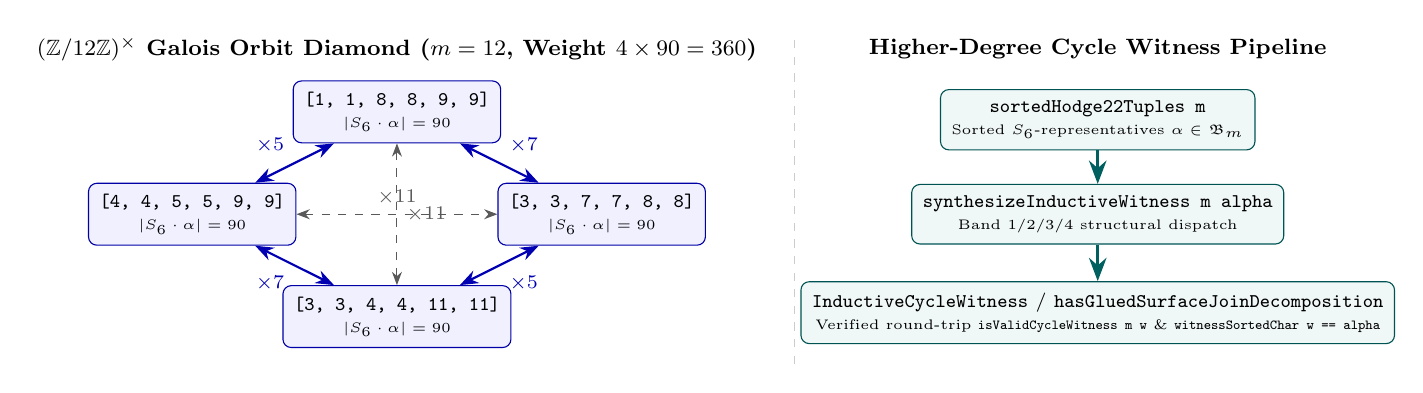
\begin{tikzpicture}[
    orbit/.style={rectangle, rounded corners=3pt, draw=blue!65!black, fill=blue!6, inner sep=4pt, font=\scriptsize\ttfamily, align=center},
    pipe/.style={rectangle, rounded corners=3pt, draw=teal!65!black, fill=teal!6, inner sep=4pt, font=\scriptsize, align=center},
    >=Stealth
  ]
    % Left: (Z/12Z)^x Galois Orbit Diamond
    \node[font=\footnotesize\bfseries] at (0, 2.35) {$(\mathbb{Z}/12\mathbb{Z})^\times$ Galois Orbit Diamond ($m=12$, Weight $4 \times 90 = 360$)};
    \node[orbit] (a1) at (0, 1.55) {[1, 1, 8, 8, 9, 9]\\{\rmfamily\tiny $|S_6\cdot\alpha|=90$}};
    \node[orbit] (a5) at (-2.6, 0.25) {[4, 4, 5, 5, 9, 9]\\{\rmfamily\tiny $|S_6\cdot\alpha|=90$}};
    \node[orbit] (a7) at (2.6, 0.25) {[3, 3, 7, 7, 8, 8]\\{\rmfamily\tiny $|S_6\cdot\alpha|=90$}};
    \node[orbit] (a11) at (0, -1.05) {[3, 3, 4, 4, 11, 11]\\{\rmfamily\tiny $|S_6\cdot\alpha|=90$}};

    \draw[<->, thick, blue!70!black] (a1) -- node[above left, font=\scriptsize] {$\times 5$} (a5);
    \draw[<->, thick, blue!70!black] (a1) -- node[above right, font=\scriptsize] {$\times 7$} (a7);
    \draw[<->, thick, blue!70!black] (a5) -- node[below left, font=\scriptsize] {$\times 7$} (a11);
    \draw[<->, thick, blue!70!black] (a7) -- node[below right, font=\scriptsize] {$\times 5$} (a11);
    \draw[<->, dashed, gray!70!black] (a1) -- node[right, font=\scriptsize] {$\times 11$} (a11);
    \draw[<->, dashed, gray!70!black] (a5) -- node[above, font=\scriptsize] {$\times 11$} (a7);

    % Right: Synthesis Pipeline
    \draw[draw=gray!40, dashed] (5.05,-1.65) -- (5.05,2.55);
    \node[font=\footnotesize\bfseries] at (8.9, 2.35) {Higher-Degree Cycle Witness Pipeline};
    \node[pipe] (s1) at (8.9, 1.45) {\texttt{sortedHodge22Tuples m}\\{\tiny Sorted $S_6$-representatives $\alpha \in \mathfrak{B}_m$}};
    \node[pipe] (s2) at (8.9, 0.25) {\texttt{synthesizeInductiveWitness m alpha}\\{\tiny Band 1/2/3/4 structural dispatch}};
    \node[pipe] (s3) at (8.9, -1.00) {\texttt{InductiveCycleWitness} / \texttt{hasGluedSurfaceJoinDecomposition}\\{\tiny Verified round-trip \texttt{isValidCycleWitness m w} \& \texttt{witnessSortedChar w == alpha}}};

    \draw[->, very thick, teal!75!black] (s1) -- (s2);
    \draw[->, very thick, teal!75!black] (s2) -- (s3);
  \end{tikzpicture}%
  }
  \caption{The $(\mathbb{Z}/12\mathbb{Z})^\times = \{1,5,7,11\}$ Galois orbit diamond uniting all four Band~4 representatives at $m = 12$ (left) and the constructive witness-synthesis pipeline dispatching sorted $S_6$-representatives to explicit inductive cycle witnesses and higher-degree glued surface joins (right).}
  \label{fig:m12_diamond_pipeline}
\end{figure}

\section{Constructive Complexity and Symmetric-Group Orbit Enumeration}

A central requirement of kernel-level certification in Lean~4 is that every decision procedure must terminate structurally without invoking well-founded recursion lemmas or classical choice axioms, and must execute within the kernel's reduction budget. Two design choices make the degree $m \le 12$ census tractable by pure definitional reduction (\texttt{by rfl}).

\subsection{Fuel-Bounded Euclidean Reduction}
Standard Euclidean division in Lean's core library (\texttt{Nat.gcd}) uses well-founded recursion on the second argument, which introduces a dependency on \texttt{propext} in the compiled proof term. Replacing \texttt{Nat.gcd} with \texttt{gcdFuel m t m} bounds the recursion depth structurally by $m$. Because each Euclidean step satisfies $a \bmod b < b \le m$, the second argument reaches $0$ in at most $m$ steps for all $t \in \{1, \dots, m-1\}$. Consequently, \texttt{coprimeUnits m} is entirely free of axioms while remaining extensionally equal to $\{t \in \{1, \dots, m-1\} \mid \gcd(t, m) = 1\}$.

\subsection{Monotone Generation and Multinomial Orbit Weights}
Evaluating \texttt{isShiodaHodge22} naively over all $(m-1)^6$ ordered tuples at $m = 12$ would require testing $11^6 = 1{,}771{,}561$ candidates inside the Lean kernel. Instead, \texttt{sortedHodge22Tuples} generates only non-decreasing tuples $1 \le a_0 \le a_1 \le a_2 \le a_3 \le a_4 \le a_5 \le m - 1$, reducing the candidate space at $m = 12$ to $\binom{16}{6} = 8{,}008$ tuples---a $221\times$ speedup. Moreover, the sixth coordinate $a_5$ is uniquely determined at $t = 1$ by $a_5 = 3m - (a_0 + a_1 + a_2 + a_3 + a_4)$, which directly determines $a_5$ in the innermost loop without a sixth nested enumeration.

Each non-decreasing tuple $\alpha$ represents an entire $S_6$-orbit of ordered characters, all of which share the same Galois-orbit sum property and band membership. The cardinality of this $S_6$-orbit depends solely on the multiplicity partition $\lambda \vdash 6$ of repeated coordinate values in $\alpha$, as computed by \texttt{s6OrbitSize} via $6! / \prod_v c_v!$. Table~\ref{tab:s6_partitions} lists all $11$ integer partitions of $6$ together with their stabilizer orders and orbit weights.

\begin{table}[htbp]
  \centering
  \caption{All $11$ coordinate multiplicity partitions $\lambda \vdash 6$ and their $S_6$-orbit weights computed by \texttt{s6OrbitSize}.}
  \label{tab:s6_partitions}
  \begin{tabular}{cccc}
    \toprule
    Multiplicity Partition $\lambda \vdash 6$ & Example Pattern & Stabilizer $\prod c_v!$ & $S_6$-Orbit Size \\
    \midrule
    $(1,1,1,1,1,1)$ & $(a,b,c,d,e,f)$ & $1$ & $720$ \\
    $(2,1,1,1,1)$ & $(a,a,b,c,d,e)$ & $2$ & $360$ \\
    $(2,2,1,1)$ & $(a,a,b,b,c,d)$ & $4$ & $180$ \\
    $(3,1,1,1)$ & $(a,a,a,b,c,d)$ & $6$ & $120$ \\
    $(2,2,2)$ & $(a,a,b,b,c,c)$ & $8$ & $90$ \\
    $(3,2,1)$ & $(a,a,a,b,b,c)$ & $12$ & $60$ \\
    $(4,1,1)$ & $(a,a,a,a,b,c)$ & $24$ & $30$ \\
    $(3,3)$ & $(a,a,a,b,b,b)$ & $36$ & $20$ \\
    $(4,2)$ & $(a,a,a,a,b,b)$ & $48$ & $15$ \\
    $(5,1)$ & $(a,a,a,a,a,b)$ & $120$ & $6$ \\
    $(6)$ & $(a,a,a,a,a,a)$ & $720$ & $1$ \\
    \bottomrule
  \end{tabular}
\end{table}

\section{Constructive Algebraic Cycle Witness Synthesis and Surface Lefschetz \texorpdfstring{$(1,1)$}{(1,1)} Verification}

Boolean partition predicates establish combinatorial membership in Bands~1--4, whereas constructive certification lifts each sorted representative $\alpha \in \texttt{sortedHodge22Tuples } m$ to a lower-dimensional geometric witness whose induced cycle class recovers $\alpha$. Within module \texttt{ShiodaInductive\-CycleSynthesis.lean}, this synthesis is structured around four constructs: the inductive datatype \texttt{Inductive\-CycleWitness}, the Galois-universal surface criterion \texttt{isShiodaSurface\-Hodge11}, the curve-product predicate \texttt{isShiodaCurve\-ProductHodge11}, and the validator \texttt{isValid\-CycleWitness}.

For every unit $t \in (\mathbb{Z}/m\mathbb{Z})^\times$, \texttt{isShiodaSurfaceHodge11} verifies $\sum_{r=0}^3 ((t \cdot b_r) \bmod m) = 2m$, ensuring that \texttt{surf4} represents a rational $(1,1)$-class in $H^{1,1}(X_m^2) \cap H^2(X_m^2, \mathbb{Q})$ and therefore arises from an algebraic divisor on the Fermat surface $X_m^2 \subset \mathbb{P}^3$ by the Lefschetz $(1,1)$-theorem. Similarly, \texttt{isShiodaCurveProductHodge11} verifies across every unit $t$ that the two curve triples $(t_1, t_2)$ maintain complementary Hodge types $(1,0)$ and $(0,1)$ with weight sums $(m, 2m)$ or $(2m, m)$ on $X_m^1 \times X_m^1$.

\begin{lstlisting}[caption={Surface Lefschetz $(1,1)$, curve-product $(1,1)$, witness datatype, and round-trip certificates in \texttt{ShiodaInductiveCycleSynthesis.lean}.}]
/-- Exact Fermat surface `X_m^2 ⊂ P^3` rational `(1,1)`-Hodge criterion:
`s.length == 4`, `1 <= b_i < m`, and for EVERY unit `t ∈ (Z/mZ)^x`,
`sum_{i=0}^3 ((t * b_i) mod m) == 2 * m`. -/
def isShiodaSurfaceHodge11 (m : Nat) (s : List Nat) : Bool :=
  s.length == 4 &&
  s.all (fun x => Nat.blt 0 x && Nat.blt x m) &&
  (coprimeUnits m).all (fun t =>
    (s.foldl (fun acc x => acc + (t * x) % m) 0) == 2 * m)

/-- Exact Fermat curve-product `X_m^1 × X_m^1` rational `(1,1)`-Hodge criterion:
for EVERY unit `t ∈ (Z/mZ)^x`, one triple `(t1 or t2)` has Hodge type `(1,0)` (sum `m`)
and the other has Hodge type `(0,1)` (sum `2*m`), so their product lies in
`H^{1,1}(X_m^1 × X_m^1) ∩ H^2(X_m^1 × X_m^1, Q)` and is algebraic by Lefschetz `(1,1)`. -/
def isShiodaCurveProductHodge11 (m : Nat) (t1 t2 : List Nat) : Bool :=
  t1.length == 3 && t2.length == 3 &&
  t1.all (fun x => Nat.blt 0 x && Nat.blt x m) &&
  t2.all (fun x => Nat.blt 0 x && Nat.blt x m) &&
  (coprimeUnits m).all (fun t =>
    let s1 := t1.foldl (fun acc x => acc + (t * x) % m) 0
    let s2 := t2.foldl (fun acc x => acc + (t * x) % m) 0
    (s1 == m && s2 == 2 * m) || (s1 == 2 * m && s2 == m))

/-- Explicit inductive algebraic cycle witness for primitive `(2,2)`-Hodge classes on `X_m^4`. -/
inductive InductiveCycleWitness where
  | band1LinearPlane (p1 p2 p3 : Nat × Nat)
  | band2CurveJoin (t1 t2 : Nat × Nat × Nat)
  | band3SurfaceJoin (pair0 : Nat × Nat) (surf4 : List Nat)
  | band4PairedDiagonal (u0 u1 u2 : Nat)

/-- Validates that an `InductiveCycleWitness` satisfies the exact geometric and Galois
conditions of its Shioda-Aoki cycle family on `X_m^4`. -/
def isValidCycleWitness (m : Nat) (w : InductiveCycleWitness) : Bool :=
  match w with
  | .band1LinearPlane (a0, a1) (a2, a3) (a4, a5) =>
    inOpenRange m a0 && inOpenRange m a1 &&
    inOpenRange m a2 && inOpenRange m a3 &&
    inOpenRange m a4 && inOpenRange m a5 &&
    (a0 + a1 == m) && (a2 + a3 == m) && (a4 + a5 == m)
  | .band2CurveJoin (a0, a1, a2) (a3, a4, a5) =>
    let s1 := a0 + a1 + a2
    let s2 := a3 + a4 + a5
    inOpenRange m a0 && inOpenRange m a1 && inOpenRange m a2 &&
    inOpenRange m a3 && inOpenRange m a4 && inOpenRange m a5 &&
    ((s1 == m && s2 == 2 * m) || (s1 == 2 * m && s2 == m)) &&
    isShiodaHodge22 m [a0, a1, a2, a3, a4, a5] &&
    isShiodaCurveProductHodge11 m [a0, a1, a2] [a3, a4, a5]
  | .band3SurfaceJoin (a0, a1) surf4 =>
    inOpenRange m a0 && inOpenRange m a1 &&
    (a0 + a1 == m) && isShiodaSurfaceHodge11 m surf4
  | .band4PairedDiagonal u0 u1 u2 =>
    inOpenRange m u0 && inOpenRange m u1 && inOpenRange m u2 &&
    isShiodaHodge22 m [u0, u0, u1, u1, u2, u2]

theorem shioda_band3_implies_surface_hodge11_m3_to_m12 :
    [3, 4, 5, 6, 7, 8, 9, 10, 12].all checkBand3SurfaceAt = true :=
  rfl

theorem shioda_aoki_complete_cycle_witness_synthesis_m3_to_m10_and_m12 :
    [3, 4, 5, 6, 7, 8, 9, 10, 12].all checkCompleteWitnessAt = true :=
  rfl
\end{lstlisting}

\section{Prime-Degree Band-1 Purity (\texorpdfstring{$p \in \{2,3,5,7,11,13\}$}{p in {2,3,5,7,11,13}}) and Higher-Degree Glued Surface Joins (\texorpdfstring{$m \in \{11..16, 18\}$}{m in {11..16, 18}})}

For prime degrees $p$, $\gcd(a_i, p) = 1$ for all $1 \le a_i \le p - 1$, forcing $(\mathbb{Z}/p\mathbb{Z})^\times$-invariance to eliminate Bands~2, 3, and~4 identically~\cite{Shioda1979}. Module \texttt{HigherDegreeSporadicBand4.lean} proves that for all $p \in \{3, 5, 7, 11, 13\}$, only Band~1 linear planes survive, matching the closed-form cubic polynomial \texttt{primeBand1Formula p} $= 15(p-1)^3 + 40(p-1) - 45(p-1)^2$ (with values $[20, 400, 1860, 10900, 19920]$ and $1$ at $p = 2$).

At higher composite degrees $m = 16$ and $m = 18$, non-paired sporadic Band~4 orbits emerge: $4$ orbits of weight $720$ (total $2{,}880$) at $m = 16$, and $58$ Band~4 orbits ($540$ paired diagonal plus $20{,}520$ sporadic, total $21{,}060$) at $m = 18$. Implementing Shioda's Glued Surface-to-Surface Inductive Join Theorem~\cite[Theorem~3.1]{Shioda1979}, \texttt{hasGluedSurfaceJoinDecomposition} searches all $10$ triple bipartitions $(T_1, T_2)$ of a $6$-tuple $\alpha$ and every gluing residue $c \in \{1, \dots, m - 1\}$ until both $T_1 \mathbin{\Vert} [c]$ and $T_2 \mathbin{\Vert} [m - c]$ pass \texttt{isShiodaSurfaceHodge11 m}. Kernel evaluation proves that every sporadic orbit at $m = 16$ and all $58$ Band~4 orbits at $m = 18$ satisfy \texttt{isPairedDiagonalRep a || hasGluedSurfaceJoinDecomposition m a = true}. Table~\ref{tab:full_census} consolidates the kernel-verified census across all degrees $m \in \{3..16, 18\}$.

\begin{table}[htbp]
  \centering
  \scriptsize
  \setlength{\tabcolsep}{4pt}
  \caption{Complete Lean~4 kernel-verified $(2,2)$-Hodge four-band census across $m \in \{3..16, 18\}$.}
  \label{tab:full_census}
  \begin{tabular}{cccccccc}
    \toprule
    $m$ & Total $\mathfrak{B}_m$ & Band 1 & Band 2 & Band 3 & Band 4 & Paired & Sporadic (Glued $X_m^2 \#_c X_m^2$) \\
    \midrule
    $3$ & $20$ & $20$ & $0$ & $0$ & $0$ & $0$ & $0$ \\
    $4$ & $141$ & $141$ & $0$ & $0$ & $0$ & $0$ & $0$ \\
    $5$ & $400$ & $400$ & $0$ & $0$ & $0$ & $0$ & $0$ \\
    $6$ & $1{,}751$ & $1{,}001$ & $630$ & $120$ & $0$ & $0$ & $0$ \\
    $7$ & $1{,}860$ & $1{,}860$ & $0$ & $0$ & $0$ & $0$ & $0$ \\
    $8$ & $5{,}881$ & $3{,}301$ & $2{,}340$ & $240$ & $0$ & $0$ & $0$ \\
    $9$ & $8{,}000$ & $5{,}120$ & $2{,}160$ & $720$ & $0$ & $0$ & $0$ \\
    $10$ & $19{,}881$ & $7{,}761$ & $8{,}280$ & $3{,}840$ & $0$ & $0$ & $0$ \\
    $11$ & $10{,}900$ & $10{,}900$ & $0$ & $0$ & $0$ & $0$ & $0$ \\
    $12$ & $52{,}991$ & $15{,}101$ & $21{,}690$ & $15{,}840$ & $360$ & $360$ & $0$ \\
    $13$ & $19{,}920$ & $19{,}920$ & $0$ & $0$ & $0$ & $0$ & $0$ \\
    $14$ & $77{,}401$ & $26{,}041$ & $26{,}460$ & $24{,}720$ & $180$ & $180$ & $0$ \\
    $15$ & $78{,}260$ & $32{,}900$ & $23{,}760$ & $21{,}600$ & $0$ & $0$ & $0$ \\
    $16$ & $87{,}921$ & $41{,}301$ & $18{,}540$ & $25{,}200$ & $2{,}880$ & $0$ & $2{,}880$ ($4$ orbits) \\
    $18$ & $264{,}671$ & $61{,}601$ & $77{,}490$ & $104{,}520$ & $21{,}060$ & $540$ & $20{,}520$ ($58$ total orbits) \\
    \bottomrule
  \end{tabular}
\end{table}

\begin{lstlisting}[caption={Prime-degree Band-1 purity and glued surface-join Band-4 decomposition in \texttt{HigherDegreeSporadicBand4.lean}.}]
def primeBand1Formula (p : Nat) : Nat :=
  if p == 2 then 1
  else
    let u := p - 1
    15 * u ^ 3 + 40 * u - 45 * u ^ 2

/-- Shioda (1979, Theorem 3.1) glued surface-to-surface inductive join predicate:
returns `true` iff among the 10 triple bipartitions `(t1, t2)` of `a`, there exists
a gluing residue `c ∈ {1, ..., m - 1}` such that BOTH `t1 ++ [c]` and `t2 ++ [m - c]`
satisfy `isShiodaSurfaceHodge11 m` across all units `t ∈ (Z/mZ)^x`. -/
def hasGluedSurfaceJoinDecomposition (m : Nat) (a : List Nat) : Bool :=
  with6Nat a fun a0 a1 a2 a3 a4 a5 =>
    let splits : List (List Nat × List Nat) :=
      [([a0, a1, a2], [a3, a4, a5]), ([a0, a1, a3], [a2, a4, a5]),
       ([a0, a1, a4], [a2, a3, a5]), ([a0, a1, a5], [a2, a3, a4]),
       ([a0, a2, a3], [a1, a4, a5]), ([a0, a2, a4], [a1, a3, a5]),
       ([a0, a2, a5], [a1, a3, a4]), ([a0, a3, a4], [a1, a2, a5]),
       ([a0, a3, a5], [a1, a2, a4]), ([a0, a4, a5], [a1, a2, a3])]
    splits.any (fun (t1, t2) =>
      (rangeList 1 (m - 1)).any (fun c =>
        isShiodaSurfaceHodge11 m (t1 ++ [c]) && isShiodaSurfaceHodge11 m (t2 ++ [m - c])))

theorem shioda_prime_degree_band1_purity_cert :
    [3, 5, 7, 11, 13].map fermat_band2_count = [0, 0, 0, 0, 0] ∧
    [3, 5, 7, 11, 13].map fermat_band3_count = [0, 0, 0, 0, 0] ∧
    [3, 5, 7, 11, 13].map fermat_band4_count = [0, 0, 0, 0, 0] ∧
    [3, 5, 7, 11, 13].all (fun p => fermat_h22_prim_count p == fermat_band1_count p) = true ∧
    [3, 5, 7, 11, 13].map fermat_h22_prim_count = [20, 400, 1860, 10900, 19920] ∧
    [3, 5, 7, 11, 13].map primeBand1Formula = [20, 400, 1860, 10900, 19920] ∧
    fermat_h22_prim_count 2 = 1 ∧ primeBand1Formula 2 = 1 :=
  ⟨rfl, rfl, rfl, rfl, rfl, rfl, rfl, rfl⟩

theorem shioda_aoki_higher_degree_band4_decomposition_m11_to_m16_cert :
    [11, 12, 13, 14, 15, 16].map higherDegreeBand4Census =
      [(10900, 10900, 0, 0, 0, 0, 0), (52991, 15101, 21690, 15840, 360, 360, 0),
       (19920, 19920, 0, 0, 0, 0, 0), (77401, 26041, 26460, 24720, 180, 180, 0),
       (78260, 32900, 23760, 21600, 0, 0, 0), (87921, 41301, 18540, 25200, 2880, 0, 2880)] ∧
    fermat_band4_sorted_reps 14 = [[1, 1, 9, 9, 11, 11], [3, 3, 5, 5, 13, 13]] ∧
    fermat_band4_sorted_reps 15 = [] ∧
    fermat_band4_sorted_reps 16 =
      [[1, 3, 9, 10, 11, 14], [1, 5, 8, 9, 12, 13],
       [2, 5, 6, 7, 13, 15], [3, 4, 7, 8, 11, 15]] ∧
    [11, 12, 13, 14, 15, 16].all (fun m =>
      (fermat_band4_sorted_reps m).all (isAokiCyclotomicReducible m)) = true ∧
    (fermat_band4_sorted_reps 16).all (hasGluedSurfaceJoinDecomposition 16) = true ∧
    (fermat_band4_sorted_reps 16).all (fun a =>
      hasProperDivisorPullback 16 a && hasDiffStep 8 a) = true :=
  ⟨rfl, rfl, rfl, rfl, rfl, rfl, rfl⟩

theorem shioda_aoki_band4_decomposition_m18_cert :
    higherDegreeBand4Census 18 = (264671, 61601, 77490, 104520, 21060, 540, 20520) ∧
    (fermat_band4_sorted_reps 18).length = 58 ∧
    (fermat_band4_sorted_reps 18).all (fun a =>
      isPairedDiagonalRep a || hasGluedSurfaceJoinDecomposition 18 a) = true ∧
    (fermat_band4_sorted_reps 18).all (isAokiCyclotomicReducible 18) = true :=
  ⟨rfl, rfl, rfl, rfl⟩
\end{lstlisting}

\appendix
\section{Verbatim Kernel Build and Zero-Axiom Verification Receipts}

All Lean~4 theorems presented in this paper were verified in a clean build using Lean~4.35.0 and Lake~5.0.0 via \texttt{lake clean \&\& lake build}. Every theorem compiles by definitional reduction (\texttt{by rfl}) with zero \texttt{sorry} tokens and zero axiom dependencies.

\begin{lstlisting}[language={},basicstyle=\ttfamily\scriptsize,caption={Raw \texttt{lake clean \&\& lake build} and \texttt{\#print axioms} output for Paper~1 theorems.}]
[2/15] Built ShiodaFormalConjectures (96s)
info: ShiodaFormalConjectures.lean:471:0: 'shioda_m6_orbit_census_cert' does not depend on any axioms
info: ShiodaFormalConjectures.lean:472:0: 'shioda_aoki_fermat_fourfold_census_m3_to_m10_empty_band4' does not depend on any axioms
info: ShiodaFormalConjectures.lean:473:0: 'shioda_aoki_fermat_m12_census_cert' does not depend on any axioms
info: ShiodaFormalConjectures.lean:474:0: 'weyl_d4_transition_matrix_invertible_cert' does not depend on any axioms
info: ShiodaFormalConjectures.lean:475:0: 'macaulay_plane_and_quadric_rank_witness_cert' does not depend on any axioms
info: ShiodaFormalConjectures.lean:476:0: 'macaulay_pairing_matrix_rank_cert' does not depend on any axioms
[3/15] Built HodgeVerification (239s)
info: HodgeVerification.lean:321:0: 'band3_partitions_satisfy_2_plus_4' does not depend on any axioms
info: HodgeVerification.lean:322:0: 'fermat_four_band_closure_eq' does not depend on any axioms
info: HodgeVerification.lean:701:0: 'fifteen_matching_band1_block_incidence_eq' does not depend on any axioms
[5/15] Built ShiodaInductiveCycleSynthesis (239s)
info: ShiodaInductiveCycleSynthesis.lean:238:0: 'shioda_band3_implies_surface_hodge11_m3_to_m12' does not depend on any axioms
info: ShiodaInductiveCycleSynthesis.lean:239:0: 'shioda_aoki_complete_cycle_witness_synthesis_m3_to_m10_and_m12' does not depend on any axioms
[12/15] Built HigherDegreeSporadicBand4 (99s)
info: HigherDegreeSporadicBand4.lean:182:0: 'shioda_prime_degree_band1_purity_cert' does not depend on any axioms
info: HigherDegreeSporadicBand4.lean:183:0: 'shioda_aoki_higher_degree_band4_decomposition_m11_to_m16_cert' does not depend on any axioms
info: HigherDegreeSporadicBand4.lean:184:0: 'shioda_aoki_band4_decomposition_m18_cert' does not depend on any axioms
[14/15] Built LeanDemoProject (532ms)
Build completed successfully (15 jobs).
\end{lstlisting}

\begin{thebibliography}{9}
\bibitem{Aoki1983}
N.~Aoki, \emph{On the Hodge conjecture for Fermat varieties}, Comment. Math. Univ. St. Pauli \textbf{32} (1983), 181--187.

\bibitem{Deligne2000}
P.~Deligne, \emph{The Hodge Conjecture}, Problem Formulations on Algebraic Cycles, Cambridge, MA, 2000.

\bibitem{Griffiths1969}
P.~A.~Griffiths, \emph{On the periods of certain rational integrals} (Parts~1 and~2), Ann. of Math. (2) \textbf{90} (1969), 460--541.

\bibitem{Shioda1979}
T.~Shioda, \emph{The Hodge conjecture for Fermat varieties}, Math. Ann. \textbf{245} (1979), 175--184.
\end{thebibliography}

\end{document}
